\documentclass[a4paper,12pt]{report}

\usepackage{alltt, fancyvrb, url}
\usepackage{graphicx}
\usepackage[utf8]{inputenc}
\usepackage{float}
\usepackage{hyperref}

\usepackage{amssymb}
\usepackage{amsmath}

% Questo commentalo se vuoi scrivere in inglese.
\usepackage[italian]{babel}

\usepackage[italian]{cleveref}

\linespread{0.97} % Imposta l'interlinea di x volte la dimensione del carattere

\title{Teoria dei numeri \\ applicata alla Crittografia}

\author{Giosuè Giocondo Mainardi\\ (n.0000933566)}
\date{\today}

\begin{document}

\maketitle

\tableofcontents
\chapter{Introduzione}
La \textbf{crittografia} è fondamentale per garantire la sicurezza delle comunicazioni digitali, proteggendo la \emph{confidenzialità, l'integrità e l'autenticità} dei dati scambiati. 
Molti degli algoritmi crittografici più diffusi e robusti si basano su solidi principi matematici derivanti dalla \textbf{teoria dei numeri}. 

Sebbene in passato crittografia e matematica fossero viste come discipline separate, con \emph{G.H. Hardy} che nel 1940 vedeva la matematica come una scienza neutra, pura e gentile,
che non si schiera e non ha applicazioni dirette, l'avvento dell'informatica ha dimostrato il loro stretto legame. 

La teoria dei numeri, con lo studio delle proprietà dei numeri interi, dei \textbf{numeri primi} e delle loro interazioni, è diventata un pilastro portante per lo sviluppo di sistemi crittografici sicuri.

La \textbf{fattorizzazione in numeri primi}, il \textbf{logaritmo discreto} e l' \textbf{algebra modulare} sono solo alcuni dei concetti chiave della teoria dei numeri che trovano 
applicazione nella crittografia moderna. Algoritmi rivoluzionari come \emph{RSA} e \emph{Diffie-Hellman}, basilari per la crittografia a chiave pubblica, sfruttano questi principi 
per garantire elevati livelli di sicurezza.  

In matematica si trovano proprietà ideali per nascondere e proteggere informazioni, come la difficoltà nel risolvere alcuni problemi aritmetici nonostante la loro apparente semplicità.

In questa relazione, si esplorerà nel dettaglio il legame inscindibile tra crittografia e teoria dei numeri, analizzando le principali applicazioni di quest'ultima nella protezione dei dati digitali. 
Si approfondiranno concetti come la Firma Digitale e le Curve Ellittiche, al fine di comprendere appieno il \textbf{ruolo cruciale} svolto dalla matematica nella \textbf{sicurezza informatica}.
%
%
%
%
\chapter{Fondamenti della teoria dei numeri}
È importante fornire prima basi teoriche matematiche per comprendere il funzionamento degli algoritmi che andremo a trattare.

La teoria dei numeri è lo studio dei numeri interi, e delle loro proprietà. L'insieme dei numeri interi è $\mathbb{Z}$ e contiene tutti i numeri interi positivi e negativi, insieme allo zero.
\begin{quote}
	\centering
	..., -5, -4, -3, -2, -1,  0,  1,  2,  3,  4,  5, ...
\end{quote}

\section{Definizioni}

\subsection*{Numero primo}
Un numero primo è un numero intero \( p > 1 \) che ha esattamente due divisori: 1 e \(p\) (se stesso).

\textbf{Esempi}: ogni numero a sinistra nella seguente tabella è primo.
\[\begin{array}{ll}
3 & = 2 + 1 \\
7 & = 2 \cdot 3 + 1 \\
31 & = 2 \cdot 3 \cdot 5 + 1 \\
211 & = 2 \cdot 3 \cdot 5 \cdot 7 + 1 \\
2311 & = 2 \cdot 3 \cdot 5 \cdot 7 \cdot 11 + 1 \\
\end{array}\]
Questo schema non continua indefinitamente, ma qualcosa di simile funziona.

Occorre però ricordare che Euclide ha dimostrato che esistono infiniti numeri primi. \cite{stein2008}

Inoltre, si fa notare che il più grande numero primo conosciuto\footnote{Largest Know Prime Number:7 dicembre 2018 da Patrick Laroche} è \[2^{82,589,933} - 1\]
e ha quasi 25 milioni di cifre.

\section{Concetti Fondamentali}
\subsection*{Fattorizzazione}
La fattorizzazione è il processo di scomposizione di un numero intero \( n \) in un prodotto di numeri primi. 

\textbf{Formalmente}: dato un numero intero \( n \), la fattorizzazione di \( n \) è data dalla rappresentazione: 
\[ n = p_1^{e_1} \cdot p_2^{e_2} \cdot \ldots \cdot p_k^{e_k} \]
dove \( p_1, p_2, \ldots, p_k \) sono numeri primi distinti e \( e_1, e_2, \ldots, e_k \) sono esponenti positivi.

\subsection*{Divisibilità e criteri di divisibilità}

Un numero \(a\) è divisibile per un numero \(b\) se il resto della divisione di \(a\) per \(b\) è zero. In altre parole, se esiste un numero intero \(k\) tale che \(a = b \cdot k\), allora \(a\) è divisibile per \(b\).

\subsection*{Massimo comune divisore (MCD)}
Il massimo comune divisore di due numeri interi \( a \) e \( b \), denotato come 
\[ \mathbb{MCD}(a, b) \] 
ed è il più grande numero intero che divide entrambi \( a \) e \( b \) senza lasciare resto.

\subsection*{Numeri coprimi}
Due numeri interi sono definiti come \textbf{coprimi} (o primi tra loro) se il loro massimo comune divisore (MCD) è uguale a 1. 

\textbf{Formalmente}: dati due numeri interi \(a\) e \(b\), essi sono coprimi se e solo se:
\[\mathbb{MCD}(a, b) = 1\]

\chapter{Aritmetica Modulare}

L'aritmetica modulare è un ramo fondamentale della teoria dei numeri che studia le operazioni aritmetiche sui resti delle divisioni intere. Questo capitolo esplora i concetti chiave dell'aritmetica modulare necessari per comprendere molti algoritmi crittografici moderni.

\section{Definizioni} 
\subsection*{Operatore modulo} Dato un numero intero $a$ e un modulo $n$, numero intero positivo, il "resto della divisione di $a$ per $n$" è il valore che rimane quando $a$ è diviso per $n$. Questo valore è sempre compreso tra 0 e $n-1$, inclusi.

Simbolicamente, possiamo esprimere il resto della divisione di $a$ per $n$ come:
\[ a \mod n \]
dove "mod" è l'operatore modulo.

\subsection*{Insieme modulo \( \mathbb{Z}_n\)}
Si sceglie un numero intero positivo \(n\), chiamato modulo, che determina l'insieme dei resti modulo \(n\). 
Questo insieme è denotato come \(\mathbb{Z}_n\)  , ed è composto da tutti i numeri interi che vanno da 0 a \(n-1\).

\textbf{Formalmente}: \[\mathbb{Z}_n = \{0, 1, 2, \ldots, n-1\}\]

\subsection*{Gruppo moltiplicativo \(\mathbb{Z}_n^*\)}
Un insieme modulo che contiene solo numeri coprimi rispetto al modulo dato è noto come gruppo moltiplicativo modulo \(n\), indicato con \(\mathbb{Z}_n^*\) o \((\mathbb{Z}/n\mathbb{Z})^*\). 
Questo gruppo è composto da tutti gli interi positivi minori di \(n\) che sono coprimi con \(n\).

\textbf{Formalmente}: \[\mathbb{Z}_n^* = \{a \in \mathbb{Z}_n : \text{MCD}(a, n) = 1\}\]

\subsection*{Funzione Totiente di Eulero} \label{sec:totiente}
La funzione totiente di Eulero, indicata con $\phi(n)$, conta il numero di interi positivi minori o uguali a $n$ che sono coprimi con $n$, ovvero che non hanno fattori comuni con $n$ eccetto $1$. 

\textbf{Formalmente}:\[\phi(n) = |\{a \in \mathbb{Z}_n : \mathbb{MCD}(a, n) = 1\}| = |\mathbb{Z}_n^*|\]
\section{Congruenza Modulare}

Data una coppia di interi $a$ e $b$, e un intero positivo $n$ detto \textbf{modulo}, diciamo che $a$ è congruo a $b$ modulo $n$, denotato come:

$$a \equiv b \pmod{n}$$

Se esistono interi $k_1$ e $k_2$ tali che:

$$a = k_1n + b$$
$$b = k_2n + a$$

In altre parole, $a$ e $b$ hanno lo stesso resto quando divisi per $n$. 

\subsection*{Classe di Resto}
L'insieme di tutti gli interi congrui a $a$ modulo $n$ è chiamato \textbf{classe di resto} o \textbf{classe di congruenza} di $a$ modulo $n$, denotata come \[[a]_n\]

\subsection*{Proprietà}
La relazione di congruenza gode delle seguenti proprietà:

\begin{enumerate}
    \item \textbf{Riflessività}: $a \equiv a \pmod{n}$ per ogni $a \in \mathbb{Z}$ e $n > 0$.
    \item \textbf{Simmetria}: Se $a \equiv b \pmod{n}$, allora $b \equiv a \pmod{n}$.
    \item \textbf{Transitività}: Se $a \equiv b \pmod{n}$ e $b \equiv c \pmod{n}$, allora $a \equiv c \pmod{n}$.
\end{enumerate}

\section{Operazioni Aritmetiche Modulari}
Le operazioni aritmetiche fondamentali (addizione, sottrazione, moltiplicazione ed esponenziazione) possono essere definite sull'insieme dei residui modulo $n$, denotato come $\mathbb{Z}_n$. Per $a, b \in \mathbb{Z}_n$:

\begin{enumerate}
    \item \textbf{Addizione modulare}:
    $$(a + b) \bmod n = r \quad \text{dove } r \in \mathbb{Z}_n \text{ è il resto della divisione di } a+b \text{ per } n$$
    
    \item \textbf{Sottrazione modulare}:
    $$(a - b) \bmod n = r \quad \text{dove } r \in \mathbb{Z}_n \text{ è il resto della divisione di } a-b \text{ per } n$$
    
    \item \textbf{Moltiplicazione modulare}:
    $$(a \cdot b) \bmod n = r \quad \text{dove } r \in \mathbb{Z}_n \text{ è il resto della divisione di } a \cdot b \text{ per } n$$
    
    \item \textbf{Esponenziazione modulare}:
    $$a^b \bmod n = r \quad \text{dove } r \in \mathbb{Z}_n \text{ è il resto della divisione di } a^b \text{ per } n$$
\end{enumerate}

Queste operazioni godono delle stesse proprietà dell'aritmetica ordinaria: commutativà per addizione e moltiplicazione, associatività, elementi neutri (0 per addizione, 1 per moltiplicazione) e inversi (modulo $n$).

\section{Inverso Moltiplicativo Modulare}

Un concetto cruciale è quello di \textbf{elemento invertibile modulo $n$}: 

un numero $a \in \mathbb{Z}_n$ è invertibile se esiste $b \in \mathbb{Z}_n$ tale che $ab \equiv 1 \pmod{n}$. $b$ è detto l'\textbf{inverso moltiplicativo} di $a$ modulo $n$, denotato come $a^{-1}$.

\subsection*{Esistenza dell'Inverso Moltiplicativo}
L'inverso moltiplicativo di $a$ modulo $n$ esiste se e solo se $a$ e $n$ sono coprimi, ovvero il loro massimo comune divisore $\mathbb{MCD}(a,n) = 1$. 

\section{Equazioni Diofantee}
Le equazioni diofantee sono equazioni polinomiali con due o più incognite che ammettono solo soluzioni intere. 
Una delle forme più semplici e utili nella crittografia è l'equazione diofantea lineare:
\[ax + by = c\]

\subsection*{Soluzioni delle Equazioni Diofantee Lineari}
Perché l'equazione $ax + by = c$ ammetta soluzioni intere, è necessario e sufficiente che $\mathbb{MCD}(a, b) = d$ divida $c$. 

In tal caso, le soluzioni sono nella forma:
\[x = x_0 + \frac{b}{d}t, \quad y = y_0 - \frac{a}{d}t\]
dove $(x_0, y_0)$ è una particolare soluzione dell'equazione e $t$ è un parametro intero.

\subsection*{Algoritmo di Euclide Esteso} \label{sec:inverso}   
Le equazioni diofantee sono necessarie per l'algoritmo di Euclide esteso, utilizzato per trovare l'inverso moltiplicativo modulo $n$.

L'algoritmo di Euclide esteso permette di risolvere l'equazione diofantea $ax + by = \mathbb{MCD}(a, b)$ e, di conseguenza, di trovare l'inverso moltiplicativo di $a$ modulo $n$. Se $a$ e $n$ sono coprimi ($\mathbb{MCD}(a, n) = 1$), esistono interi $x$ e $y$ tali che:
\[ax + ny = 1\]
In questo caso, $x$ è l'inverso moltiplicativo di $a$ modulo $n$, ossia:
\[a \cdot x \equiv 1 \pmod{n}\]

\section{Aritmetica Modulare sui Numeri Primi}

Le proprietà dell'aritmetica modulare si semplificano notevolmente quando il modulo $n$ è un numero primo $p$. In questo caso, l'insieme $\mathbb{Z}_p$ è un \textbf{campo}, ovvero ogni elemento non nullo è invertibile (\( |\mathbb{Z}_p| =|\mathbb{Z}_p^*| \)).

\subsubsection*{Piccolo Teorema di Fermat} \label{sec:fermat}
Espressione generale, dato $p$ primo e $a$ intero::
$$a^p \equiv a \pmod{p} \quad \forall a \in \mathbb{Z}$$

Questo teorema viene utilizzato anche come Test di Primalità di un numero, è spesso espresso in un'altra forma equivalente, con \(a\) che è un intero coprimo con \(p\):

\[a^{p-1} \equiv 1 \pmod{p}\quad,\quad con\quad \mathbb{MCD}(a,p)=1\]

\subsubsection*{Teorema di Eulero (Fermat generalizzato)}

$$a^{\phi(n)} \equiv 1 \pmod{n} \quad \text{se } \mathbb{MCD}(a,n) = 1$$

Dove $\phi(n)$ è la \textbf{funzione totiente di Eulero}, che conta il numero di interi positivi minori di $n$ e coprimi con $n$.

\subsection*{Teorema Cinese del Resto (CRT)} \label{sec:cinese}
Il teorema cinese del resto è un importante risultato della teoria dei numeri che permette di risolvere un sistema di congruenze simultanee. 

Supponiamo di avere un sistema di congruenze lineari:
\[\begin{cases}
x \equiv a_1 \pmod{m_1} \\
x \equiv a_2 \pmod{m_2} \\
\vdots \\
x \equiv a_n \pmod{m_n}
\end{cases}\]

dove $a_1, a_2, \ldots, a_n$ sono gli interi dati e $m_1, m_2, \ldots, m_n$ sono gli interi positivi coprimi a due a due.

Il teorema cinese del resto afferma che esiste una soluzione unica modulo $M = m_1 \cdot m_2 \cdot \ldots \cdot m_n$ per il sistema di congruenze. In altre parole, esiste un unico intero $x$ tale che $x \equiv a_i \pmod{m_i}$ per ogni $i$.

La soluzione $x$ può essere calcolata utilizzando l'algoritmo del teorema cinese del resto, che coinvolge l'utilizzo dell'inverso moltiplicativo modulo $m_i$ per ogni $i$.

Il teorema cinese del resto è ampiamente utilizzato in crittografia e in altri campi della matematica applicata, in particolare quando si lavora con grandi numeri e sistemi di congruenze complessi.
%
%
%
%
%
%
%
%
%
%
%
%
%
%
%
%
%
%
%
%
%
%
%
%
%
%
%
%
%
%
%
%
%
%
%
%
%
%
%
%
%
\chapter{Il Cifrario RSA}
Il cifrario RSA, introdotto dai crittografi Ron Rivest, Adi Shamir e Leonard Adleman nel 1977, rappresenta uno dei più importanti e diffusi algoritmi crittografici a chiave pubblica. 
Esso sfrutta le proprietà della teoria dei numeri e dell'aritmetica modulare per garantire la sicurezza delle comunicazioni. 
A differenza dei sistemi crittografici a chiave simmetrica, in cui la stessa chiave viene utilizzata per cifrare e decifrare i messaggi, il cifrario RSA utilizza due chiavi diverse, una pubblica e una privata.

\section{Principi Fondamentali}
Il cifrario RSA si basa su due principi fondamentali:

\begin{enumerate}
    \item La \textbf{difficoltà computazionale} di fattorizzare grandi numeri interi composti. Questo problema, noto come "problema della fattorizzazione intera", è uno dei problemi più difficili in teoria dei numeri e in crittografia. Anche se non è stato dimostrato essere NP-hard\footnote[1]{NP-hard significa che un problema è almeno tanto difficile quanto il problema più difficile in NP (nondeterministic polynomial time).}, non si conosce alcun algoritmo efficiente in grado di risolverlo in tempi ragionevoli per numeri sufficientemente grandi.
    \item La \textbf{facilità relativa di calcolare esponenziali modulari}, operazione che sta alla base del processo di cifratura e decifratura. Infatti, questa può essere eseguita in modo efficiente tramite tecniche come l'esponenziazione veloce.
\end{enumerate}

\section{Generazione delle Chiavi}
La generazione delle chiavi nel cifrario RSA segue i seguenti passi:

\begin{enumerate}
    \item Scegliere due numeri primi distinti $p$ e $q$ di grandi dimensioni.
    \item Calcolare $n = p \cdot q$, dove $n$ è chiamato modulo. La dimensione di $n$ determina la sicurezza del sistema crittografico.
    \item Calcolare $\phi(n) = (p - 1)(q - 1)$, dove $\phi$ è la funzione totiente di Eulero, vedi \ref{sec:totiente}.
    \item Scegliere un numero intero $e$ tale che $1 < e < \phi(n)$ e $\operatorname{MCD}(e, \phi(n)) = 1$. Il numero $e$ è chiamato esponente di cifratura. Tipicamente, si sceglie un valore piccolo per $e$, come $65537$ \footnote{Numero primo ha pochi bit impostati a 1, cosa che velocizza l'elaborazione}, per rendere più efficienti le operazioni di cifratura.
    \item Determinare $d$ tale che $d \cdot e \equiv 1 \pmod{\phi(n)}$. Il numero $d$ è chiamato esponente di decifratura. Esso può essere calcolato usando l'algoritmo di Euclide esteso, come specificato in \ref{sec:inverso}.
\end{enumerate}

La coppia $(e, n)$ rappresenta la chiave pubblica, mentre $(d)$ è la chiave privata. La chiave pubblica può essere ampiamente diffusa, mentre la chiave privata deve essere mantenuta segreta.

\subsection*{Scelta di Numeri Primi Robusti}
La sicurezza del cifrario RSA dipende in modo cruciale dalla difficoltà di fattorizzare il modulo $n$, che è il prodotto dei due numeri primi $p$ e $q$. Pertanto, è fondamentale scegliere numeri primi ``robusti'' o ``forti'' per $p$ e $q$, in modo da resistere agli attacchi di fattorizzazione.

Un numero primo è considerato ``robusto'' se soddisfa determinate proprietà che lo rendono più resistente agli attacchi di fattorizzazione. Alcune di queste proprietà includono:

\begin{itemize}
    \item \textbf{Dimensione adeguata}: I numeri primi $p$ e $q$ devono avere dimensioni sufficientemente grandi, successivamente si approfondisce.
    \item \textbf{Struttura specifica}: Alcune forme speciali di numeri primi, come i numeri primi di Sophie Germain, sono considerate più resistenti agli attacchi di fattorizzazione.
    \item \textbf{Test di primalità avanzati}: Per verificare l'effettiva primalità di $p$ e $q$, è necessario utilizzare test di primalità avanzati, che sono più robusti rispetto al semplice test di primalità di Fermat, vedi \ref{sec:fermat}.
\end{itemize}

Tra i test di primalità avanzati più utilizzati, possiamo menzionare:

\begin{enumerate}
    \item \textbf{Test di Miller-Rabin}: Questo test probabilistico è in grado di determinare se un numero è composto con un alto grado di precisione. Esegue una serie di test basati sul Piccolo Teorema di Fermat e sul fatto che, se $n$ è composto, esistono sempre radici non banali dell'unità modulo $n$.
    \item \textbf{Test di Solovay-Strassen}: Anche questo è un test probabilistico che sfrutta il fatto che, se $n$ è composto, esistono sempre radici non banali dell'unità modulo $n$. Il test di Solovay-Strassen è più efficiente del test di Miller-Rabin per numeri molto grandi.
\end{enumerate}

Entrambi questi test possono essere eseguiti più volte per aumentare la probabilità di rilevare correttamente se un numero è primo o composto. Inoltre, possono essere combinati con altri criteri, come la verifica delle proprietà dei numeri primi sicuri o di Sophie Germain, per ottenere numeri primi ancora più robusti.

È importante sottolineare che, nonostante l'utilizzo di numeri primi robusti e test di primalità avanzati, la sicurezza del cifrario RSA dipende anche da altri fattori, come la gestione sicura delle chiavi e la corretta implementazione dell'algoritmo.

\subsection*{Specifiche Attuali dimensioni Chiavi RSA}

Ecco le specifiche attuali per la lunghezza delle chiavi RSA:

\begin{itemize}
    \item \textbf{1024 bit}: Considerata insicura per la maggior parte degli scopi. Non è più raccomandata per l'uso.
    \item \textbf{2048 bit}: Attualmente considerata sicura per la maggior parte degli scopi. Raccomandata per molti utilizzi.
    \item \textbf{3072 bit}: Fornisce un margine di sicurezza maggiore, utilizzata per esigenze di sicurezza più elevate.
    \item \textbf{4096 bit}: Utilizzata per esigenze di sicurezza molto elevate, anche se comporta operazioni più lente.
\end{itemize}

Queste raccomandazioni sono in linea con le linee guida fornite da organizzazioni come il NIST (National Institute of Standards and Technology)\cite{nist}.

\section{Cifratura e Decifratura}
Sia $m$ il messaggio in chiaro, rappresentato come un numero intero nel range $[0, n - 1]$. Per trasformare il messaggio in un numero intero, si possono utilizzare varie tecniche di codifica, come la rappresentazione ASCII o Unicode dei caratteri.

\begin{enumerate}
    \item La cifratura avviene calcolando $c \equiv m^e \pmod{n}$, dove $c$ è il testo cifrato.
    \item La decifratura avviene calcolando $m \equiv c^d \pmod{n}$.
\end{enumerate}

La sicurezza del cifrario RSA risiede nella difficoltà computazionale di fattorizzare $n$ in $p$ e $q$, dato che la conoscenza di $p$ e $q$ permette di calcolare $\phi(n)$ e quindi la chiave privata $d$. Pertanto, la scelta di numeri primi $p$ e $q$ sufficientemente grandi è cruciale per garantire la sicurezza del sistema.

\section{Applicazioni e Sicurezza del Cifrario RSA}

Il cifrario RSA è utilizzato per crittografare, firma digitale, scambio di chiavi e autenticazione, inclusi protocolli come SSL/TLS e PGP. Tuttavia, la sicurezza dipende dalla difficoltà di fattorizzare numeri composti. Con l'aumento della potenza di calcolo, potrebbe essere necessario aumentare le dimensioni delle chiavi. Sono presenti potenziali vulnerabilità legate alla scelta dei numeri primi e alla gestione delle chiavi, quindi è importante seguire le best practice di sicurezza.

\section{Varianti e applicazioni}
Il cifrario RSA è stato esteso e modificato in varie forme per migliorare le sicurezza e le prestazioni. Si presentano solo alcune varianti e applicazioni del cifrario RSA:

\subsection{RSA Three Marsenne prime} \cite{padmaja2016}
Variante dell'algoritmo RSA che sfrutta il Teorema Cinese dei Resti (CRT), vedi \ref{sec:cinese}, per migliorare l'efficienza computazionale durante le operazioni di cifratura e decifratura, utilizzando tre numeri primi di Marsenne per la generazione del modulo RSA.

\subsubsection*{Numeri di Marsenne}
I numeri di Marsenne sono numeri primi \(p\) tali che anche \(2^p - 1\) è un numero primo. 

\subsubsection*{Differenze nella generazione Chiave}
\begin{itemize}
    \item Genera tre numeri primi di Marsenne distinti $p$, $q$, e $r$ di lunghezza simile.
    \item Calcola $n = p \cdot q \cdot r$ e $\phi(n) = (p-1)(q-1)(r-1)$.
\end{itemize}

\subsection{RSA con Esponenti Brevi e Bilanciati} \cite{10.1007/978-3-540-30580-4_14}
Variante dell'algoritmo RSA che mira a ridurre i costi computazionali durante le operazioni di cifratura e decifratura, utilizzando esponenti più corti e bilanciati.

\subsubsection*{Generazione della chiave}
\begin{enumerate}
    \item Genera due numeri primi distinti $p$ e $q$ di lunghezza simile.
    \item Calcola $n = pq$ e $\phi(n) = (p-1)(q-1)$.
    \item Scegli gli esponenti pubblici $e_1$, $e_2$ tali che $e_1 + e_2 = \phi(n) + 1$ e $\mathbb{MCD}(e_1, \phi(n)) = \mathbb{MCD}(e_2, \phi(n)) = 1$.
    \item Calcola $d_1 \equiv e_1^{-1} \pmod{\phi(n)}$ e $d_2 \equiv e_2^{-1} \pmod{\phi(n)}$.
\end{enumerate}
La chiave pubblica è $(n, e_1, e_2)$ e la chiave privata è $(d_1, d_2)$.

\subsubsection*{Cifratura}
\begin{enumerate}
    \item Separa $m$ in due parti $m_1$ e $m_2$ tali che $m = m_1 \cdot m_2 \bmod n$.
    \item Cifra le due parti $c_1 \equiv m_1^{e_1} \bmod n$ e $c_2 \equiv m_2^{e_2} \bmod n$.
    \item $c = c_1 \cdot c_2 \bmod n$.
\end{enumerate}

\subsubsection*{Decifratura}
\begin{enumerate}
    \item Decifra le due parti $m_1 \equiv c^{d_1} \bmod n$ e $m_2 \equiv c^{d_2} \bmod n$.
    \item Combina $m_1$ e $m_2$ per ottenere $m \equiv m_1 \cdot m_2 \bmod n$.
\end{enumerate}

L'idea chiave di questa variante è che gli esponenti $e_1$ ed $e_2$ sono molto più corti dell'esponente $e$ utilizzato nel RSA standard, riducendo così i costi computazionali durante la cifratura e la decifrazione.

\subsection{RPrime RSA} \cite{Nasution_2020}
Rprime migliora il costo computazionale sul lato della decifrazione combinando RSA a Esponenti Brevi Bilanciati e RSA Three Prime. 
La sicurezza di Rprime RSA, così come quella di RSA riequilibrato, dipende dalla sicurezza offerta dall'esponente privato d e dalle dimensioni dei primi utilizzati.
\subsubsection*{Generazione della chiave}
\begin{enumerate}
\item Genera $k$ numeri primi distinti $p_1, p_2, \ldots, p_k$ tali che $\mathbb{MCD}(p_i - 1, p_j - 1) = 2$ per $1 \leq i, j \leq k$.
\item Calcola $n = p_1 \cdot p_2 \cdots p_k$ e $\phi(n) = (p_1 - 1)(p_2 - 1) \cdots (p_k - 1)$.
\item Genera $k$ numeri casuali $d_{p_1}, d_{p_2}, \ldots, d_{p_k}$ tali che $\mathbb{MCD}(d_{p_i}, p_i - 1) = 1$ e $d_{p_i} \equiv d_{p_j} \pmod{2}$ per $1 \leq i, j \leq k$.
\item Calcola $d$ usando il Teorema dei Resti Cinesi (CRT).
\item Calcola $e \equiv d^{-1} \pmod{\phi(n)}$.
\end{enumerate}
La chiave pubblica è $(e, n)$ e la chiave privata è $(p_1, \ldots, p_k, d_{p_1}, \ldots, d_{p_k}, d)$.

\subsection{Multi-factor RSA} \cite{Nasution_2020}
Il Multi-factor RSA si basa sulla modifica della struttura del RSA , con \(n = pqr\) o \(n = p^2 r\). 
Nel processo di generazione delle chiavi, viene dato un parametro aggiuntivo chiamato b. 

\subsubsection*{Generazione della chiave}
\begin{enumerate}
\item Genera $b$ numeri primi distinti $p_1, p_2, \ldots, p_b$.
\item Calcola $n = p_1 \cdot p_2 \cdots p_b$.
\item Calcola $\phi(n) = (p_1 - 1)(p_2 - 1) \cdots (p_b - 1)$.
\item Scegli lo stesso $e$ usato nella chiave pubblica RSA standard, cioè $e = 65537$. Quindi calcola $d \equiv e^{-1} \pmod{\phi(n)}$.
\end{enumerate}
La chiave pubblica è $(e, n)$ e la chiave privata è $(d)$.

\subsubsection*{Decifrazione}
La cifratura avviene come nel RSA standard, mentre la decifratura no, si decripta il messaggio usando il Teorema dei Resti Cinesi (CRT):
\begin{enumerate}
\item Calcola $d_i \equiv d \bmod (p_i - 1)$ e $m_i \equiv c^{d_i} \bmod p_i$ per ogni $i$, $1 \leq i \leq b$.
\item Combina gli $m_i$ usando il CRT per ottenere $M \equiv c^d \bmod n$.
\end{enumerate}

\subsection{RSA a Chiave Multipla}
Il sistema RSA a chiave multipla consente di utilizzare più di due chiavi per cifrare e decifrare i messaggi, aumentando la sicurezza e la flessibilità del sistema. In questo schema, viene generato un insieme di $t$ chiavi pubbliche $(e_1, n_1), (e_2, n_2), \ldots, (e_t, n_t)$ e un'unica chiave privata $d$ condivisa.

La cifratura avviene calcolando:
\[c \equiv m^{e_1 e_2 \cdots e_t} \pmod{n_1 n_2 \cdots n_t}\]

Mentre la decifratura si ottiene calcolando:
\[m \equiv c^d \pmod{n_1 n_2 \cdots n_t}\]

Questo schema offre una maggiore sicurezza rispetto al RSA tradizionale, in quanto un potenziale attaccante dovrebbe fattorizzare il prodotto di tutti i moduli $n_i$ per compromettere il sistema.

\subsection{RSA in Sistemi Crittografici Ibridi}
La crittografia ibrida combina il cifrario RSA con algoritmi di crittografia simmetrica, sfruttando i punti di forza di entrambi i sistemi. In questo schema, RSA viene utilizzato per cifrare una chiave simmetrica casuale, che a sua volta viene impiegata per cifrare il messaggio vero e proprio con un algoritmo simmetrico più efficiente.

Questo approccio offre diversi vantaggi, come una maggiore efficienza nelle operazioni di cifratura e decifratura dei dati, una migliore gestione delle chiavi e una maggiore sicurezza complessiva del sistema. 

Esempi di schemi ibridi includono PGP (Pretty Good Privacy) e S/MIME (Secure/Multipurpose Internet Mail Extensions).

\subsection{RSA a Chiave Condivisa}
Sebbene il cifrario RSA sia principalmente utilizzato come sistema a chiave pubblica, esiste anche una variante a chiave condivisa, nota come RSA a chiave segreta. In questo schema, Alice e Bob concordano su una chiave segreta comune $(e, n)$, dove $n$ è il prodotto di due numeri primi segreti $p$ e $q$, ed $e$ è l'esponente di cifratura.

La cifratura e la decifratura avvengono come nel RSA standard, ma utilizzando la stessa chiave $(e, n)$ condivisa. Questo approccio offre maggiore efficienza rispetto al RSA a chiave pubblica, ma richiede un canale sicuro per lo scambio della chiave segreta.
%
%
%
%
%
%
%
%
%
%
%
%
%
%
%
%
%
\chapter{Il Problema del Logaritmo Discreto}
Il problema del logaritmo discreto è uno dei problemi fondamentali nella crittografia a chiave pubblica e nella teoria dei numeri. Esso costituisce la base di molti importanti algoritmi crittografici, come il crittosistema di Diffie-Hellman, il DSA (Digital Signature Algorithm) e i crittosistemi basati sulle curve ellittiche.

\begin{figure}[ht]
    \centering
    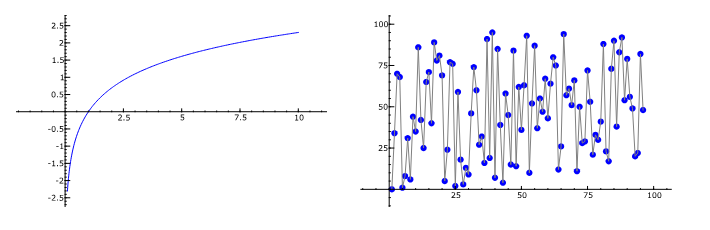
\includegraphics[width=1.0\textwidth]{img/logarithms.png}
    \caption{Confronto tra logaritmo continuo e logaritmo discreto \cite{stein2008}.}
    \label{fig:logarithms}
\end{figure}

\section{Fondamenti teoria dei gruppi}
Per comprendere il problema del logaritmo discreto, è necessario avere una conoscenza di base della teoria dei gruppi.

\subsection*{Gruppo}

Un gruppo \( (G, \cdot) \) è un insieme \( G \) di elementi con a un'operazione binaria \( \cdot \) che soddisfa le seguenti proprietà:

\begin{enumerate}
    \item \textbf{Chiusura}: \(\forall a, b \in G, \, \quad a \cdot b \in G.\)
    \item \textbf{Associatività}: \(\forall a, b, c \in G, \quad (a \cdot b) \cdot c = a \cdot (b \cdot c).\)
    \item \textbf{Elemento neutro}: \(\exists e \in G \quad tale \quad che \quad \forall a \in G, e \cdot a = a \cdot e = a.\)
    \item \textbf{Elemento inverso}: \(\forall a \in G, \quad \exists b \in G \quad tale \quad che \quad a \cdot b = b \cdot a = e.\)
\end{enumerate}

\subsection*{Gruppo Ciclico}

Un gruppo ciclico è un gruppo \( (G, \cdot) \) generato da un singolo elemento \( g \). Ogni elemento del gruppo può essere scritto come una potenza (o multiplo) di \( g \). Formalmente, un gruppo \( G \) è ciclico se esiste \( g \in G \) tale che
\[G = \langle g \rangle = \{ g^k \mid k \in \mathbb{Z} \}.\]

\subsection*{Gruppo Ciclico Finito}

Un gruppo ciclico finito è un gruppo ciclico \( (G, \cdot) \) con un numero finito di elementi. Se \( G \) è generato da \( g \), allora esiste un intero positivo \( n \) tale che gli elementi di \( G \) sono
\[\{e, g, g^2, g^3, \ldots, g^{n-1}\},\]
dove \( e \) è l'elemento neutro e \( g^n = e \). La cardinalità (o ordine) del gruppo ciclico finito è \( n \).

\subsection*{Gruppo abeliano}
Un gruppo abeliano è un gruppo \( (G, \cdot) \) che soddisfa anche la 
\subsubsection*{Commutatività (Proprietà di Abel):} \[ \forall a, b \in  G, \quad a + b = b + a \].


\section{Definizione Formale}
Sia $G$ un gruppo ciclico finito di ordine $n$, con generatore $g$. Per ogni elemento $h \in G$, esiste un unico intero $x$, con $0 \leq x < n$, tale che:
\[h = g^x\]

L'intero $x$ è chiamato logaritmo discreto di $h$ rispetto alla base $g$ nel gruppo $G$, e si indica con:
\[x = \log_g h\]

Il \textbf{problema del logaritmo discreto} consiste nel calcolare $x$ dati $g$, $h$ e $G$. 

\section{Proprietà e Applicazioni}
Il problema del logaritmo discreto gode di alcune importanti proprietà che lo rendono fondamentale nella crittografia:

\begin{itemize}
    \item Calcolare $g^x$ dato $g$ e $x$ è un'operazione \textbf{relativamente semplice }da eseguire in modo efficiente.
    \item Al contrario, calcolare $x$ dati $g$ e $g^x$ è un \textbf{problema computazionalmente difficile} per gruppi sufficientemente grandi.
    \item La \textbf{difficoltà del problema} dipende dalla dimensione del gruppo e dalla scelta del generatore $g$.
\end{itemize}

\section{Algoritmi di Calcolo}
Nonostante la difficoltà intrinseca del problema del logaritmo discreto, sono stati sviluppati diversi algoritmi per tentare di risolverlo in modo efficiente. Alcuni dei più noti includono:
\begin{itemize}
    \item \textbf{Algoritmo baby-step giant-step}: tecnica efficiente che riduce la complessità da esponenziale a radice quadrata, ma che richiede grande quantità di memoria, vedi \cite{silverman2009elliptic} e \cite{coron2011baby}.
    \item \textbf{Algoritmo rho di Pollard}: algoritmo probabilistico che sfrutta la ricerca di sequenze di esponenti nel gruppo, vedi \cite{nickerson2020collision}.
\end{itemize}

Tuttavia, per gruppi sufficientemente grandi, questi algoritmi non sono in grado di risolvere il problema del logaritmo discreto in tempi ragionevoli. Questa proprietà è fondamentale per garantire la sicurezza dei sistemi crittografici basati su tale problema.
%
%
%
%
%
%
%
%
%
%
%
%
%
%
\chapter{Algoritmo Diffie-Hellman}
L'algoritmo Diffie-Hellman, introdotto nel 1976 dai crittografi Whitfield Diffie e Martin Hellman, rappresenta un protocollo rivoluzionario per lo scambio sicuro di chiavi crittografiche su un canale non protetto. Esso consente a due parti di stabilire una chiave segreta condivisa senza dover trasmettere la chiave stessa sul canale di comunicazione, rendendo così impossibile per un potenziale ascoltatore intercettare la chiave.

L'algoritmo Diffie-Hellman si basa sul problema del logaritmo discreto, un problema matematico computazionalmente difficile, per garantire la sicurezza della chiave scambiata.

\section{Descrizione dell'Algoritmo}

Supponiamo che Alice e Bob vogliano stabilire una chiave segreta condivisa per comunicare in modo sicuro. Il protocollo Diffie-Hellman si svolge come segue:

\begin{enumerate}
    \item Alice e Bob concordano pubblicamente due numeri primi: un numero primo grande $p$ e un generatore $g$ dell'ordine $p$.
    \item Alice sceglie un numero intero casuale $a$ come sua chiave privata, calcola $A = g^a \bmod p$ e invia $A$ a Bob.
    \item Bob sceglie un numero intero casuale $b$ come sua chiave privata, calcola $B = g^b \bmod p$ e invia $B$ ad Alice.
    \item Alice calcola la chiave segreta condivisa $K = B^a \bmod p$.
    \item Bob calcola la stessa chiave segreta condivisa $K = A^b \bmod p$.
\end{enumerate}

È possibile dimostrare che $K$ calcolato da Alice e Bob è lo stesso valore:

\begin{align*}
K &= B^a \bmod p \\
  &= (g^b)^a \bmod p \\
  &= g^{ab} \bmod p \\
  &= (g^a)^b \bmod p \\
  &= A^b \bmod p
\end{align*}

\section{Sicurezza dell'Algoritmo}
La sicurezza dell'algoritmo Diffie-Hellman risiede nella difficoltà computazionale di calcolare il logaritmo discreto, ovvero di trovare $a$ o $b$ dati $g$, $p$, $A$ e $B$. Un potenziale ascoltatore che intercetti $A$ e $B$ non sarebbe in grado di derivare la chiave segreta condivisa $K$ senza conoscere $a$ o $b$.

Inoltre, è importante scegliere valori sufficientemente grandi per $p$ e $g$, in modo da rendere il problema del logaritmo discreto computazionalmente intrattabile con le risorse di calcolo attuali.

\section{Applicazioni e Utilizzo}
L'algoritmo Diffie-Hellman ha avuto un impatto significativo sulla crittografia moderna e sulla sicurezza delle comunicazioni. Esso è ampiamente utilizzato in numerosi protocolli crittografici e di sicurezza, come SSL/TLS, IPsec e SSH, per stabilire chiavi segrete condivise prima di iniziare una comunicazione crittografata ("handshake").

Inoltre, l'algoritmo Diffie-Hellman è alla base di altri importanti sistemi crittografici, come il Digital Signature Algorithm (DSA) e la crittografia a curva ellittica (ECC).

\section{Considerazioni Finali}
\begin{itemize}
    \item \textbf{Non è completo:} Diffie-Hellman permette lo scambio sicuro di chiavi, ma non cifra direttamente i dati o firma i messaggi. È necessario combinare DH con altri algoritmi crittografici.
    
    \item \textbf{Richiede gestione accurata:} È essenziale gestire attentamente i parametri e le chiavi per un'implementazione sicura di Diffie-Hellman.
    
    \item \textbf{Prevenzione degli attacchi:} Devono essere adottate misure per prevenire attacchi side-channel e altri vettori di attacco durante l'implementazione di Diffie-Hellman.
\end{itemize}

Inoltre, l'implementazione pratica dell'algoritmo Diffie-Hellman richiede una gestione accurata dei parametri crittografici e delle chiavi, nonché l'adozione di contromisure per prevenire potenziali attacchi side-channel o altre fonti di attacco.
%
%
%
%
%
%
\chapter{Curve Ellittiche}
Le curve ellittiche sono insiemi di punti $(x, y)$ che soddisfano un'equazione di forma cubica: $y^2 = x^3 + ax + b$, dove $a$ e $b$ sono costanti. Le curve ellittiche hanno molte applicazioni in crittografia grazie alla loro proprietà di essere non solo additive ma anche moltiplicative.

\section{Prerequisiti}
\textbf{Definizione:} Un campo \( (F, +, \cdot) \) è un insieme non vuoto \( F \) con due operazioni binarie \( + \) e \( \cdot \) che soddisfano le seguenti proprietà:
\begin{enumerate}
    \item \( (F, +) \) è un gruppo abeliano con elemento neutro \( 0 \).
    \item \( (F \setminus \{0\}, \cdot) \) è un gruppo abeliano con elemento neutro \( 1 \).
    \item La moltiplicazione è distributiva rispetto all'addizione.
\end{enumerate}

Ad esempio, se \( p \) è un numero primo, allora \( \mathbb{Z}_p\) è un campo.

\section{Definizione}
Una curva ellittica su un campo $K$ è l'insieme dei punti $(x, y)$ che soddisfano l'equazione:
\[y^2 = x^3 + ax + b\]

dove $a, b \in K$ e $4a^3 + 27b^2 \neq 0$. Il punto all'infinito $\mathcal{O}$ è incluso nella curva ellittica.

\section{Operazioni su Curve Ellittiche}
Le curve ellittiche supportano operazioni di somma e moltiplicazione tra punti. L'operazione di somma tra due punti $P$ e $Q$ su una curva ellittica restituisce un terzo punto $R$ che giace sulla stessa curva. L'operazione di moltiplicazione tra un punto $P$ e uno scalare $k$ restituisce un punto $Q$ che è la somma di $P$ con se stesso $k$ volte.

\section{Crittoanalisi delle Curve Ellittiche}
Le curve ellittiche sono utilizzate in crittografia per la loro resistenza a diverse tecniche di crittoanalisi, come l'attacco brute-force e l'attacco conosciuto come "baby-step giant-step". Tuttavia, la sicurezza delle curve ellittiche dipende dalla scelta dei parametri e dalla corretta implementazione degli algoritmi crittografici.

\section{Applicazioni delle Curve Ellittiche}
Le curve ellittiche sono utilizzate in diversi protocolli crittografici, come il Diffie-Hellman ellittico (ECDH) per lo scambio di chiavi segrete, l'algoritmo di firma digitale ellittica (ECDSA) per la firma digitale e il crittosistema di ElGamal ellittico per la crittografia a chiave pubblica. Le curve ellittiche sono anche utilizzate in applicazioni come la crittografia di dispositivi mobili e la sicurezza delle transazioni finanziarie.

\section{Diffie-Hellman Ellittico (ECDH)}
Variante del Diffie-Hellman adattata alle curve ellittiche per stabilire una chiave segreta condivisa su un canale non sicuro.

\subsection*{Scambio di Chiavi con ECDH}
Alice e Bob concordano sui parametri della curva ellittica $(a, b, p)$ e un punto base $G$. Alice sceglie $a$, Bob sceglie $b$. Si scambiano $A = aG$ e $B = bG$, quindi calcolano $K = abG$.

\subsection*{Vantaggi e Applicazioni}
L'ECDH offre maggiore efficienza e sicurezza computazionale rispetto al Diffie-Hellman tradizionale. È utilizzato in TLS, SSH e IPsec e come base per ECDSA e ElGamal ellittico.

%
%
%
%
%
%
\chapter{Firma Digitale}
La firma digitale è un meccanismo crittografico fondamentale per garantire l'autenticità, l'integrità e la non-ripudiabilità dei dati digitali. Essa svolge un ruolo analogo a quello della firma autografa nei documenti cartacei, ma sfrutta tecniche di crittografia a chiave pubblica per offrire maggiore sicurezza e verificabilità. I principali algoritmi utilizzati per la firma digitale sono il Digital Signature Algorithm (DSA) e il cifrario RSA.
\section{Funzioni Hash}
Le funzioni hash sono essenziali per il funzionamento delle firme digitali.

In questa sezione, si introducono i concetti chiave delle funzioni hash necessari per comprendere come esse siano utilizzate nella firma digitale.

\subsection*{Definizione di Funzione Hash Crittografica}
Le funzioni hash crittografiche sono un sottoinsieme specifico delle funzioni hash, progettate e analizzate per soddisfare determinati requisiti di sicurezza crittografica. 
Una funzione hash è una funzione matematica che mappa un input di lunghezza arbitraria a un output di lunghezza fissa, chiamato \textit{digest} o \textit{hash value}.

\textbf{Formalmente}: una funzione hash crittografica $H$ può essere definita come segue:
\[H: \{0,1\}^* \rightarrow \{0,1\}^n\]

dove $\{0,1\}^*$ rappresenta l'insieme di tutte le stringhe binarie di lunghezza arbitraria e $\{0,1\}^n$ rappresenta l'insieme delle stringhe binarie di lunghezza fissa $n$.

\subsection*{Proprietà Fondamentali}

Per essere utilizzata nella firma digitale, una funzione hash deve possedere le seguenti proprietà fondamentali:

\begin{itemize}
    \item \textbf{Resistenza alla preimmagine}: Dato un valore hash $h$, dovrebbe essere computazionalmente infeasible trovare un input $x$ tale che $H(x) = h$.
    \item \textbf{Resistenza alla seconda preimmagine}: Dato un input $x_1$, dovrebbe essere computazionalmente infeasible trovare un altro input $x_2$ tale che $x_1 \neq x_2$ e $H(x_1) = H(x_2)$.
    \item \textbf{Resistenza alle collisioni}: Dovrebbe essere computazionalmente infeasible trovare due input distinti $x_1$ e $x_2$ tali che $H(x_1) = H(x_2)$.
\end{itemize}

\subsection*{Funzioni Hash Crittografiche Comuni}
\begin{itemize}
    \item \textbf{MD5 (Message Digest Algorithm 5)}: una delle funzioni hash più conosciute, MD5 produce un output di 128 bit. Tuttavia, a causa di vulnerabilità crittografiche scoperte, MD5 non è più considerata sicura per molte applicazioni critiche.
    \item \textbf{SHA-1 (Secure Hash Algorithm 1)}: produce un output di 160 bit ed è stata ampiamente utilizzata in passato. Analogamente a MD5, ha subito critiche e attacchi, rendendola inadeguata per applicazioni sicure.
    \item \textbf{SHA-2 (Secure Hash Algorithm 2)}: una famiglia di funzioni hash che include SHA-224, SHA-256, SHA-384 e SHA-512, con numeri che indicano la dimensione dell'output in bit. SHA-2 è attualmente considerata sicura ed è ampiamente utilizzata in molte applicazioni crittografiche.
    \item \textbf{SHA-3 (Secure Hash Algorithm 3)}: la più recente famiglia di funzioni hash standardizzata dal NIST. SHA-3 è stata progettata come alternativa a SHA-2, con una struttura crittografica diversa basata su Keccak, offrendo robustezza contro una vasta gamma di attacchi.
\end{itemize}

\section{Firma Digitale con RSA}
Il cifrario RSA può essere utilizzato per realizzare un meccanismo di firma digitale robusto e sicuro, sfruttando le sue proprietà matematiche.

\subsection*{Generazione della Firma Digitale con RSA}
Nel cifrario RSA, ogni utente ha una coppia di chiavi: una chiave pubblica $(e, n)$ e una chiave privata $d$, dove $n$ è il prodotto di due numeri primi $p$ e $q$, $e$ è l'esponente di cifratura e $d$ è l'esponente di decifratura tale che:
\[d \cdot e \equiv 1 \pmod{\phi(n)}\]
Per firmare un messaggio $m$, il mittente:

\begin{enumerate}
    \item Calcola l'impronta digitale $H(m)$ del messaggio $m$ utilizzando una funzione di hash crittografica.
    \item Cifra l'impronta digitale $H(m)$ con la chiave privata $d$, ottenendo la firma digitale $s$:
    \[ s \equiv H(m)^d \pmod{n}\]
\end{enumerate}

\subsection*{Verifica della Firma Digitale con RSA}
Per verificare la firma digitale $s$, il destinatario:

\begin{enumerate}
    \item Calcola l'impronta digitale $H(m)$ del messaggio ricevuto $m$.
    \item Decifra la firma digitale $s$ con la chiave pubblica $(e, n)$ del mittente:
    \[v \equiv s^e \pmod{n}\]
    \item Se $v = H(m)$, la firma digitale è valida.
\end{enumerate}

\begin{figure}[ht]
    \centering
    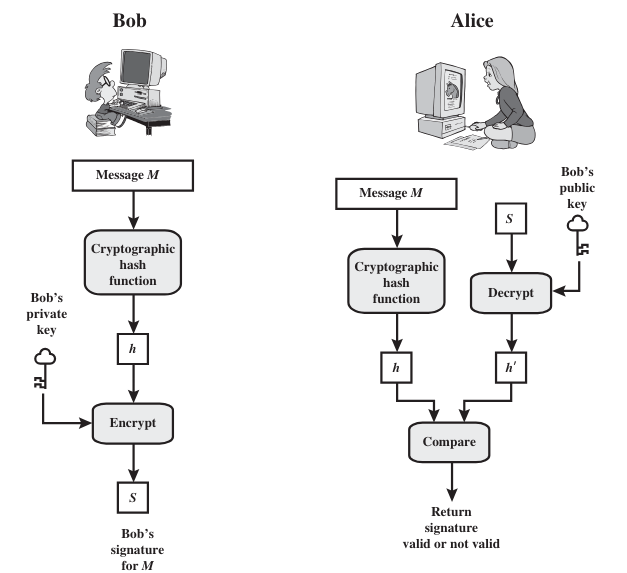
\includegraphics[width=0.8\textwidth]{img/digital_signature_process.png}
    \caption{Processo di Firma Digitale dal libro \cite{stallings2011cryptography}}
    \label{fig:digital_signature_process}
\end{figure}

\section{Firma Digitale con DSA}
Il Digital Signature Algorithm (DSA) è uno standard per la firma digitale di documenti elettronici basato sul problema del logaritmo discreto.

\subsection*{Generazione della Firma Digitale con DSA}
Siano $p$ un numero primo grande, $q$ un fattore primo di $p - 1$, e $g$ un generatore dell'ordine $q$ nel campo $\mathbb{Z}_p^*$. Sia $x$ la chiave privata del mittente e $y = g^x \bmod p$ la corrispondente chiave pubblica.

Per firmare un messaggio $m$, il mittente calcola un valore casuale $k$ coprime con $q$ e determina:

\begin{align*}
r &= (g^k \bmod p) \bmod q \\
s &= k^{-1}(H(m) + xr) \bmod q
\end{align*}

Dove $H(m)$ è l'impronta digitale del messaggio $m$ e $(k^{-1} \bmod q)$ è l'inverso moltiplicativo di $k$ modulo $q$. La firma digitale è la coppia $(r, s)$.

\subsection*{Verifica della Firma Digitale con DSA}
La verifica della firma avviene calcolando:
\[v = g^{H(m)}y^{rs} \bmod p \bmod q\]

Se $v = r$, la firma è valida.

\section{Sicurezza e Utilizzo}
La sicurezza della firma digitale con DSA risiede nella difficoltà di calcolare il logaritmo discreto $x$ dato $g$ e $y$, mentre per RSA dipende dalla difficoltà di fattorizzare il modulo $n$. Inoltre, la funzione di hash crittografica deve essere resistente alle collisioni.

La firma digitale trova ampio utilizzo in diversi contesti per garantire l'autenticità, l'integrità e la non-ripudiabilità dei dati digitali. Alcune modalità d'utilizzo comuni includono:

\begin{itemize}
    \item Transazioni Elettroniche
    \item Certificazione di Documenti
    \item Protezione del Software
    \item Autenticazione dei Messaggi di Posta Elettronica
\end{itemize}

Queste sono solo alcune delle modalità d'utilizzo della firma digitale, che trova applicazione in molti altri contesti in cui è necessario garantire l'autenticità e l'integrità dei dati digitali. Standard come SSL/TLS, S/MIME e PGP incorporano meccanismi di firma digitale..
%
%
%
%
%
%
%
%
%
%
%
%

\chapter{Firma Digitale Ellittica (ECDSA)}
La Firma Digitale Ellittica è uno schema di firma digitale basato sulle curve ellittiche. Consente di garantire autenticità, integrità e non-ripudiabilità dei dati digitali attraverso l'utilizzo di tecniche a chiave pubblica.

\section{Generazione delle Chiavi}
Nel sistema ECDSA, ogni utente ha una coppia di chiavi: una chiave privata $d$ e una corrispondente chiave pubblica $Q$, calcolate come segue:

\begin{enumerate}
    \item Scegliere una curva ellittica $E$ su un campo finito $\mathbb{F}_p$ e un punto base $G$ sulla curva.
    \item Scegliere un numero intero casuale $d$ come chiave privata, con $1 \leq d \leq n-1$, dove $n$ è l'ordine del punto base $G$.
    \item Calcolare la chiave pubblica $Q = dG$.
\end{enumerate}

La chiave privata è $(d)$ , mentre la chiave pubblica $Q$.

\section{Generazione della Firma Digitale}

Per firmare un messaggio $m$, il mittente segue questi passi:

\begin{enumerate}
    \item Scegliere un valore casuale $k$ tale che $\mathsf{MCD}(k, n) = 1$, dove $n$ è l'ordine del punto base $G$ sulla curva ellittica.
    
    \item Calcolare il punto $kG$ ottenuto moltiplicando il punto base $G$ per lo scalare $k$. Quindi, calcolare $r$ come la coordinata $x$ di questo punto $kG$:
    \[r = (kG)_x \bmod n\]
    Dove $(kG)_x$ indica la coordinata $x$ del punto $kG$ sulla curva ellittica.
    
    \item Calcolare $s = k^{-1}(H(m) + dr) \bmod n$, dove $H(m)$ è l'impronta digitale del messaggio $m$ ottenuta tramite una funzione di hash crittografica e $d$ è la chiave privata del mittente.
\end{enumerate}

La firma digitale del messaggio $m$ è la coppia $(r, s)$.

\section{Verifica della Firma Digitale}
Per verificare la firma digitale $(r, s)$ di un messaggio $m$, il destinatario deve:

\begin{enumerate}
    \item Calcolare $w = s^{-1} \bmod n$.
    \item Calcolare $u_1 = H(m)w \bmod n$ e $u_2 = rw \bmod n$.
    \item Calcolare $X = u_1G + u_2Q$.
    \item Se $X_x = r \bmod n$, dove $X_x$ è la coordinata $x$ del punto $X$, la firma digitale è valida.
\end{enumerate}

\section{Sicurezza e Proprietà}
La sicurezza dell'ECDSA risiede nella difficoltà computazionale di risolvere il problema del logaritmo discreto ellittico, ovvero di trovare $d$ dati $G$ e $Q$. Un potenziale attaccante che conoscesse $d$ sarebbe in grado di generare firme digitali valide, compromettendo l'integrità del sistema.

Inoltre, la funzione di hash crittografica utilizzata per calcolare l'impronta digitale del messaggio deve essere resistente alle collisioni e alle preimmagini, in modo da garantire l'unicità delle firme digitali.

\section{Applicazioni e Standard}
L'ECDSA è stato adottato come standard per la firma digitale da parte di numerosi enti e organizzazioni, tra cui il NIST \cite{nist}. Usato per la firma di documenti elettronici, l'autenticazione dei messaggi di posta elettronica e le transazioni finanziarie elettroniche.

Inoltre, è stato incorporato in diversi protocolli crittografici e standard di sicurezza, come SSL/TLS, S/MIME e PGP.


\nocite{*}
\bibliographystyle{plain}
\bibliography{report-template}

\end{document}
